\section{Обоснование исследования и приложения алгоритмов компьютерного зрения в антропометрии}

В задаче математического моделирования тела человека на основе бесконтактных антропометрических измерений важнейшую роль играет синтез различных подходов, включая алгоритмы обнаружения объекта, алгоритмы извлечения признаков, алгоритмы классификации объектов. Разработка систем компьютерного зрения в антропометрии является целью данного диссертационного исследования.


Алгоритмы и методы компьютерного зрения являются не только необходимыми для создания системы программного обеспечения, но и для дальнейшего изучения преимуществ каждого алгоритма и метода, составляя теоретическую важность развития данного направления научных исследований. Для достижения высокой эффективности и скорости обработки видеоданных необходимо сочетание с другими алгоритмами. Условием выбора простого алгоритма является быстрая скорость обработки, которая удовлетворяет реальные потребности системы и сохраняет при этом ее точность.

Исследование алгоритмов и методов в области компьютерного зрения требует процесса анализа и оценки преимуществ и недостатков каждого алгоритма и метода. Необходимо четкое понимание структур системных операций, эффективность и точность каждого этапа всей системы. Нужно четко проанализировать систему, чтобы правильно выбрать алгоритм.

Автоматизация процесса извлечения антропометрических признаков (расположение и размер каждой части человеческого тела, как описано на (рис. \ref{img1})) является важным элементом эффективной работы всей системы. Результатом извлечения антропометрических признаков являются входные данные для классификации объектов и создания приложений для смартфонов.

Данные со статических изображений и видео, факторы окружающей среды (ограничения по разрешению камеры и шуму условия регистрации, включая освещение, траекторию и скорость движения камеры и пр.) будут влиять на этапы обработки, поэтому следует выбрать алгоритм, чтобы уменьшить влияние объективных факторов и сосредоточиться на объекте, подлежащем обработке. Надо подробно описывать важные части объекта для более точной и эффективной работы системы. 

Целью работы была разработка автоматизированной измерительной системы, основанной на изображениях и видео на смартфоне. Эта система использует методы и алгоритмы обработки изображений и машинного обучения компьютерного зрения.

Наша система состоит из трех основных частей: извлечение антропометрических признаков, процессы обучения и тестирования, классификация новых данных (рис. \ref{img7}). Новизна нашего подхода заключаются в следующих пунктах:

\begin{itemize}
	\item Классификация антропометрических признаков на основе алгоритмов машинного обучения;
	\item Разработка программного комплекса бесконтактной антропометрии для смартфона;
	\item Создание 3D-модели человеческого тела на основе полученных антропометрических признаков.
\end{itemize}
\begin{figure}[ht!]
\centering
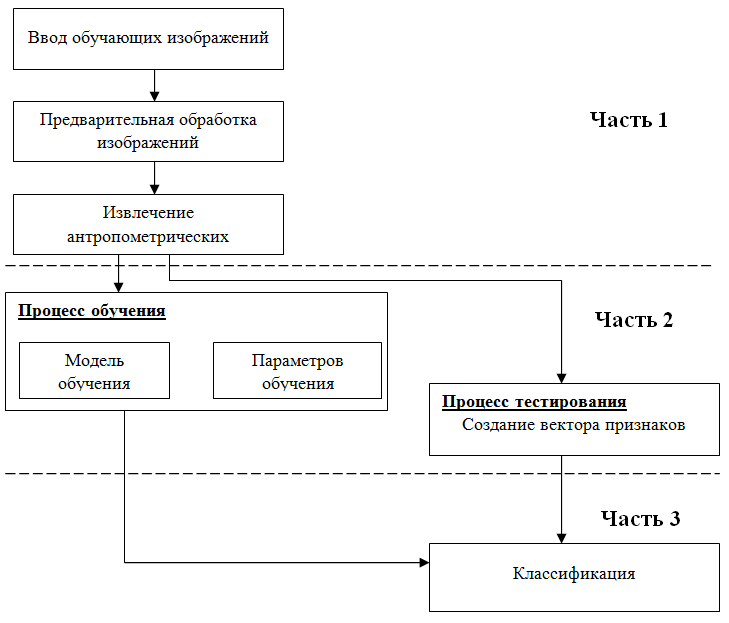
\includegraphics [scale=0.8] {images/h7.png}
\begin{center}
%\captionsetup{justification=justified, labelsep=period}
\caption{Блок-схема антропометрической системы} \label{img7}
\end{center}
\end{figure}
Система предназначена для использования в различных областях, таких как интернет-магазины для помощи пользователям в выборе размера одежды и фитнес-приложения.